W pełni funkcjonalne, wieloplatformowe PHP IDE zbudowane na bazie IntelliJ IDEA firmy JetBrains. Został on zaprojektowany specjalnie w celu ułatwienia rozwoju aplikacji internetowych napisanych w PHP. Dostarcza wszystkie narzędzia i funkcje dla PHP i obsługuje technologie frontendowe.
Znakomicie radzi sobie z dużymi projektami, podpowiadaniem składni, oraz debugowaniem.
Na dzień dzisiejszy środowisko to jest bezkonkurencyjne. Jest to rozwiązanie płatne jednak z wieloma zniżkami czy też darmowymi wersjami dla studentów.

\begin{figure}[H]
    \centering
    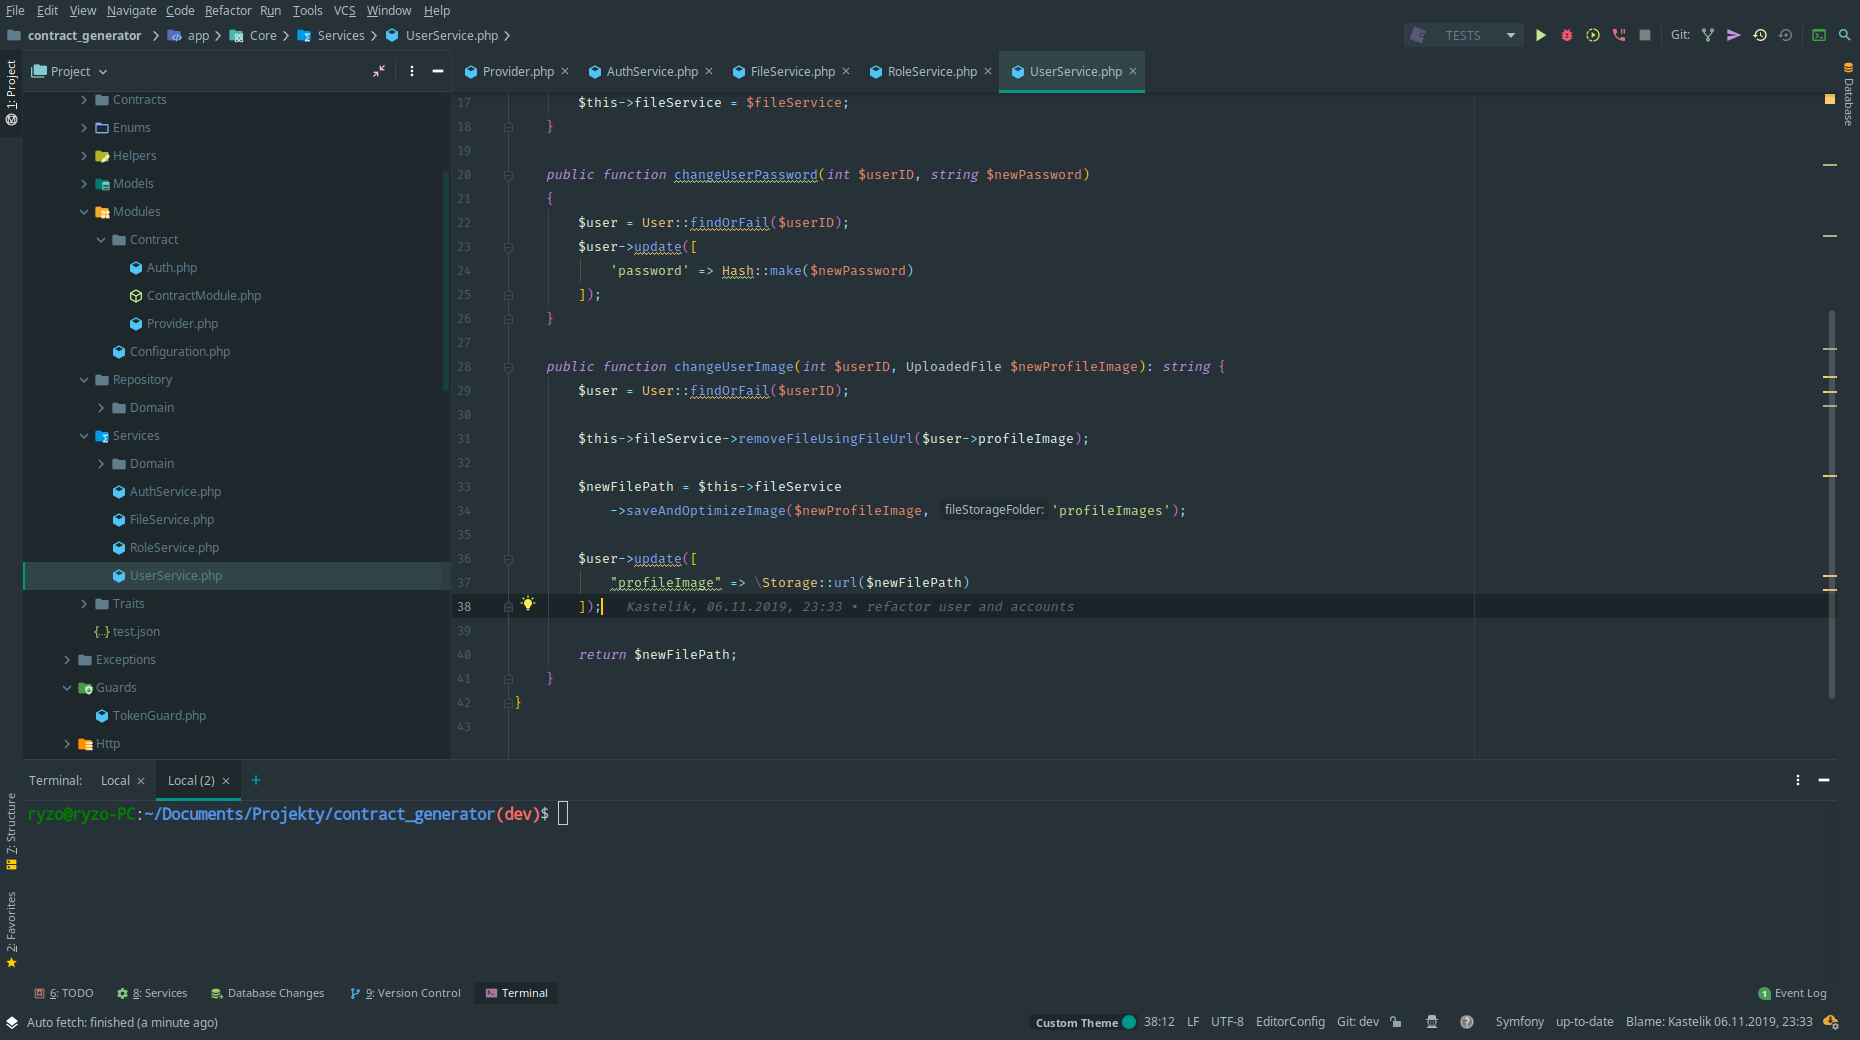
\includegraphics[width=6in]{images/phpstorm.png}
    \caption{Wygląd IDE  w projekcie \label{fig:phpstorm}}
\end{figure}